\documentclass[a4paper,11pt]{article}

\usepackage[empty]{fullpage}
\usepackage{titlesec}
\usepackage[usenames,dvipsnames]{color}
\usepackage{enumitem}
\usepackage{fancyhdr}
\usepackage[english]{babel}
\usepackage{tabularx}
\usepackage{fontawesome5}
\usepackage{multicol}
\usepackage{graphicx}
\usepackage[export]{adjustbox}
\usepackage[sfdefault]{roboto}
\usepackage[hidelinks]{hyperref}
\usepackage{montserrat}


\setlength{\multicolsep}{3.0pt}
\setlength{\columnsep}{5pt}

% Adjust footer
\pagestyle{fancy}
\fancyhf{} % clear all header and footer fields
\renewcommand{\headrulewidth}{0pt}
\renewcommand{\footrulewidth}{0pt}
\setlength{\footskip}{5pt} % Increase footskip to resolve fancyhdr warning

% Adjust margins
\addtolength{\oddsidemargin}{-0.5in}
\addtolength{\evensidemargin}{-0.5in}
\addtolength{\textwidth}{1.0in}
\addtolength{\topmargin}{-.7in}
\addtolength{\textheight}{1.3in}

\urlstyle{same}

\raggedbottom
\raggedright
\setlength{\tabcolsep}{0in}

% Sections formatting
\titleformat{\section}{
	\vspace{-6pt}\scshape\raggedright\large\bfseries
}{}{0em}{}[\color{black}\titlerule \vspace{-7pt}]

% Ensure that generate pdf is machine readable/ATS parsable
\pdfgentounicode=1

% Custom commands
\newcommand{\resumeItem}[1]{
	\item\small{#1 \vspace{-2pt}}
}

\newcommand{\resumeSubheading}[4]{
	\vspace{-2pt}\item
		\begin{tabular*}{0.97\textwidth}[t]{l@{\extracolsep{\fill}}r}
			\textbf{#1} & \textbf{\small #2} \\
			\textit{\small#3} & \textit{\small #4} \\
		\end{tabular*}\vspace{-7pt}
}

\newcommand{\resumeProjectHeading}[2]{
		\item
		\begin{tabular*}{0.97\textwidth}{l@{\extracolsep{\fill}}r}
			\small#1 & \textbf{\small #2} \\
		\end{tabular*}\vspace{-7pt}
}

\newcommand{\resumeSubHeadingListStart}{\begin{itemize}[leftmargin=0.15in, label={}]}
\newcommand{\resumeSubHeadingListEnd}{\end{itemize}}
\newcommand{\resumeItemListStart}{\begin{itemize}}
\newcommand{\resumeItemListEnd}{\end{itemize}\vspace{-5pt}}

\begin{document}

\begin{minipage}[c]{0.15\textwidth}
	\fbox{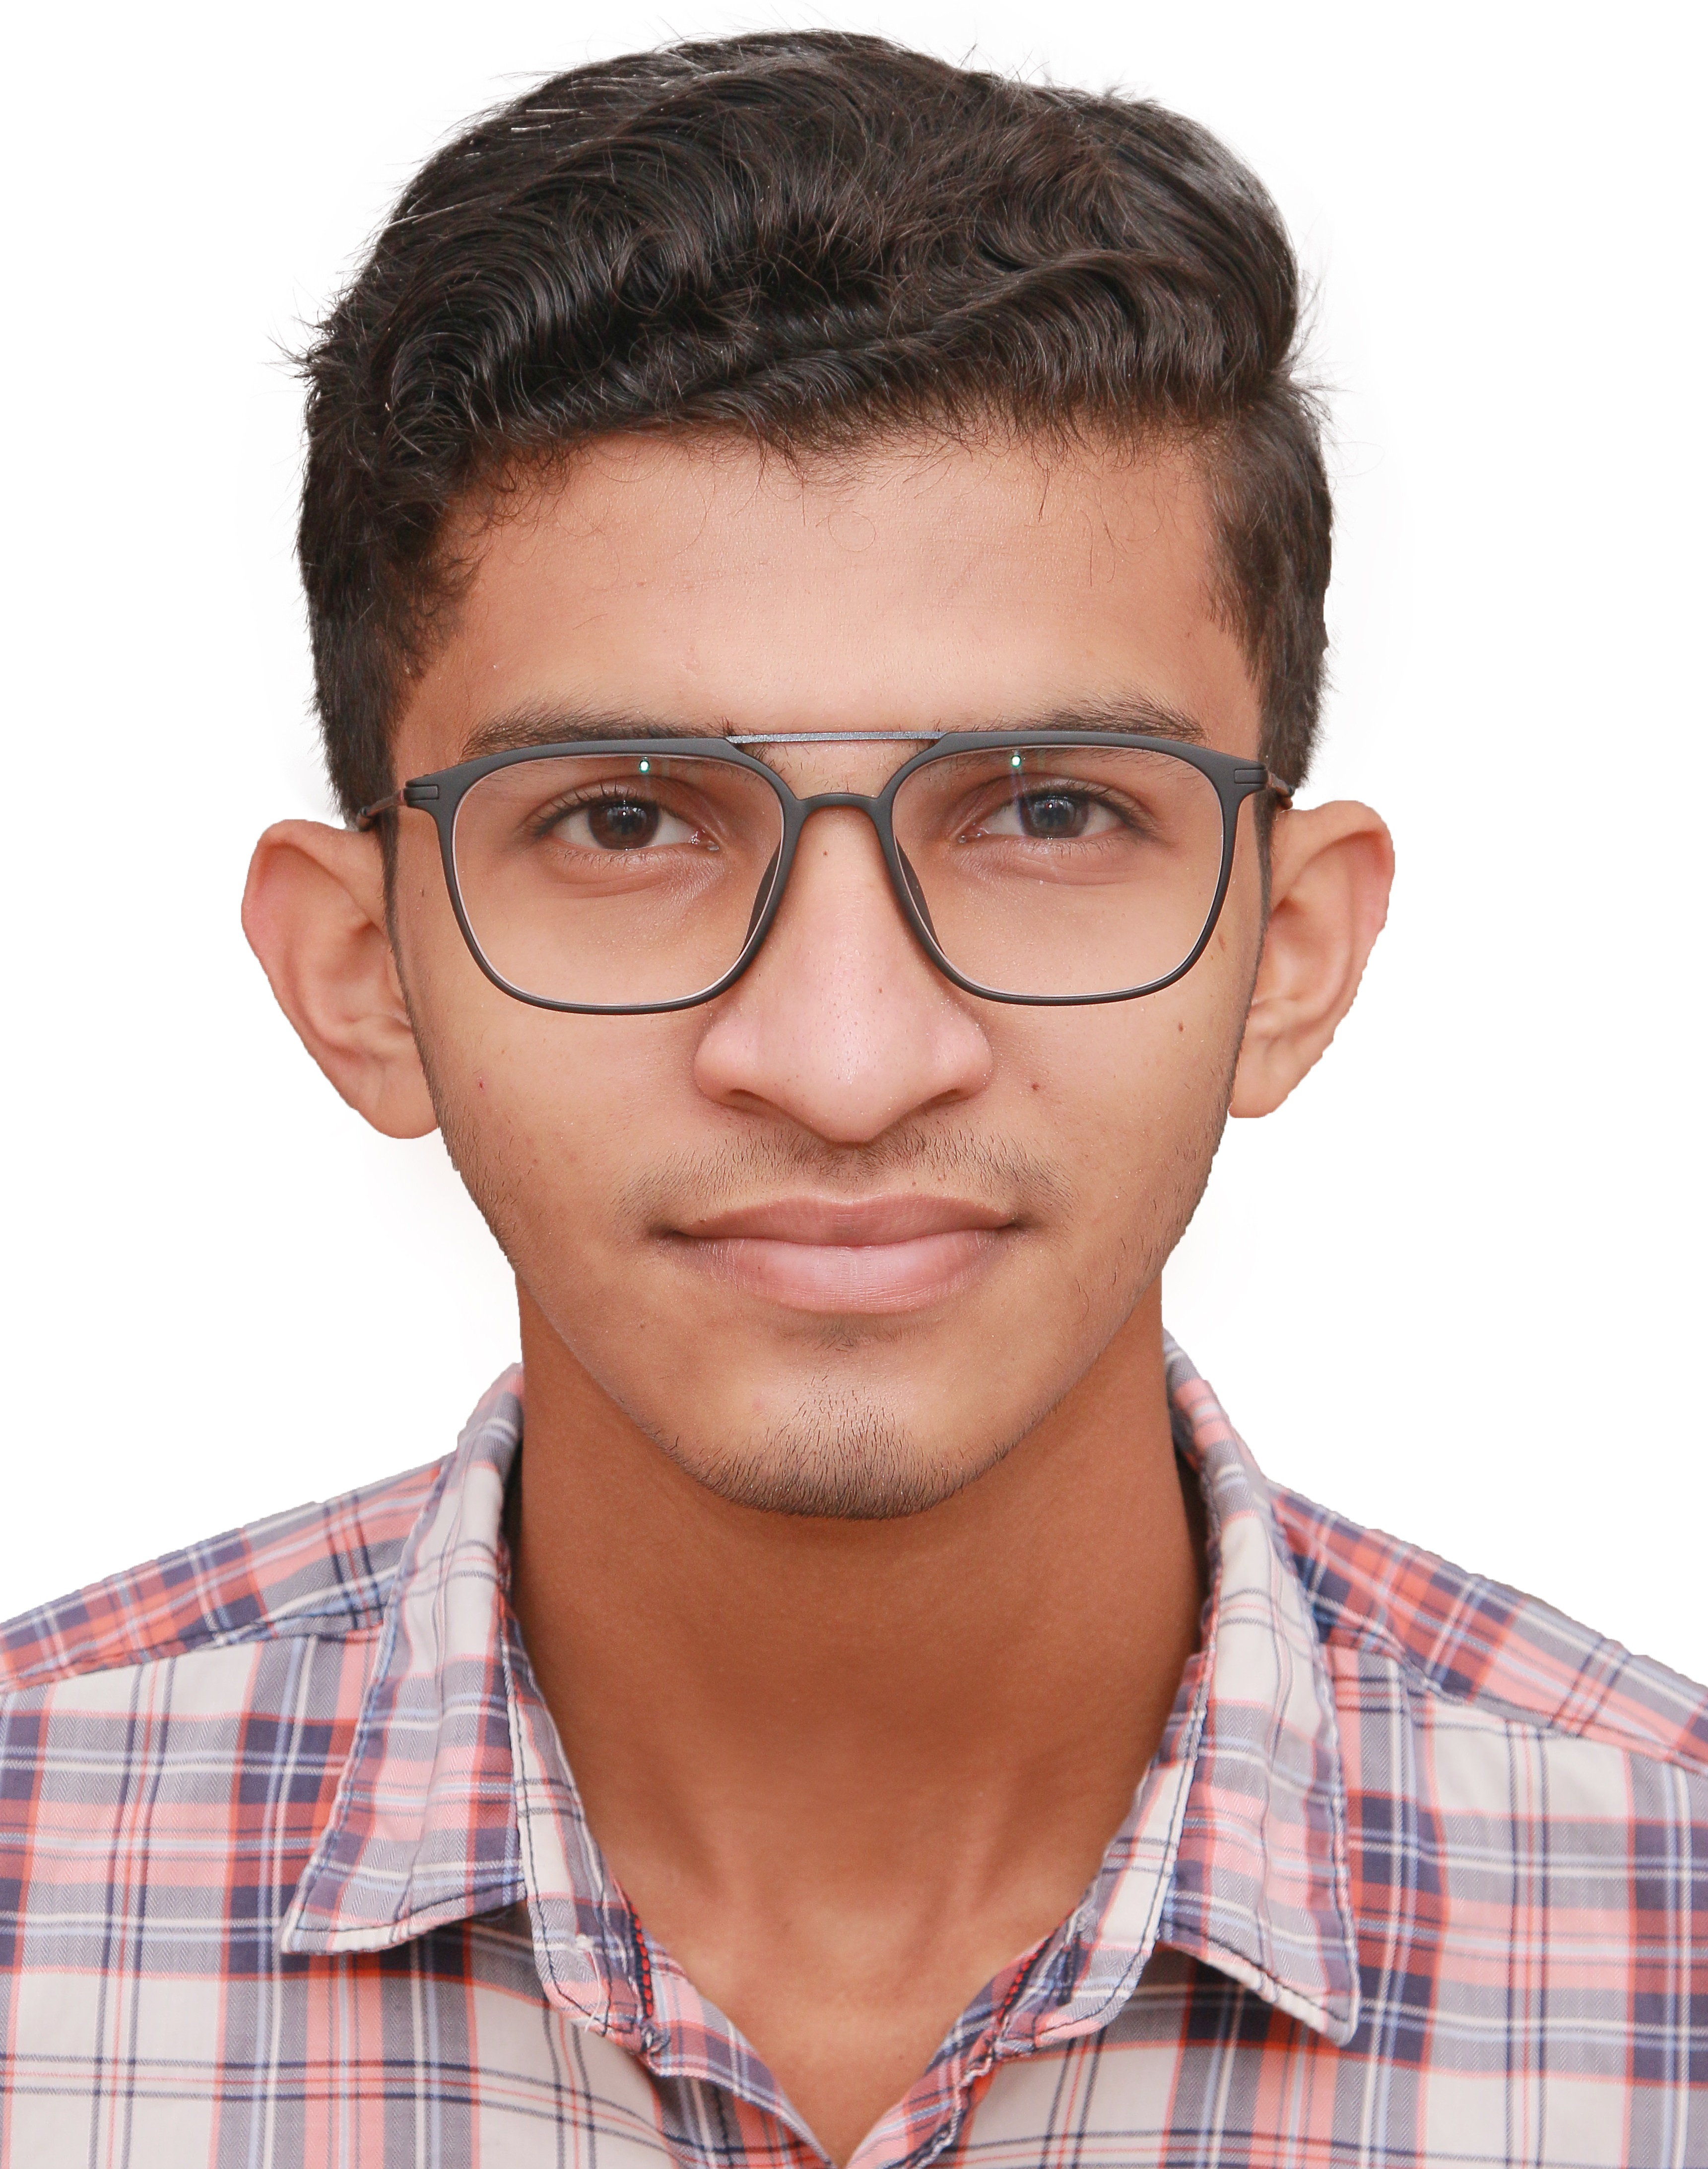
\includegraphics[width=0.84\textwidth]{photo.jpg}}
\end{minipage}
\begin{minipage}[t]{0.84\textwidth}  % Adjusted width to fill space
	\begin{center}
		{\fontfamily{Montserrat-TOsF}\selectfont \textbf{\Huge \scshape \href{https://ajmalbuv.github.io}{Ajmal Basheer}}} \\ \vspace{1pt}
		\small{
			\raisebox{-0.1\height}\faPhone\ \href{tel:+919496444520}{\underline{+91 9496444520}} $|$
			\raisebox{-0.2\height}\faEnvelope\ \href{mailto:ajmalbuv@gmail.com}{\underline{ajmalbuv@gmail.com}} $|$
			\raisebox{-0.2\height}\faLinkedin\ \href{https://linkedin.com/in/ajmalbuv}{\underline{linkedin.com/ajmalbuv}} $|$
			\raisebox{-0.2\height}\faGithub\ \href{https://github.com/ajmalbuv}{\underline{github.com/ajmalbuv}}
		}
	\end{center}
\end{minipage}


\section{Summary}
\begin{itemize}[leftmargin=0.15in, label={}]
	\small{\item{
				Full-stack developer with expertise in Python, Django, PostgreSQL, and Flutter. Experienced in designing and deploying scalable applications with optimized performance and security. Proven ability to enhance system efficiency, streamline development workflows, and contribute to high-availability cloud deployments. Passionate about delivering high-quality software solutions in dynamic IT environments.
				}}
\end{itemize}
\section{Education}
\resumeSubHeadingListStart
\resumeSubheading
{Krupanidhi Degree College}{Bengaluru, Karnataka}
{Bachelor of Computer Applications}{Aug. 2021 -- July 2024}
\resumeSubheading
{MIC Higher Secondary School}{Malappuram, Kerala}
{Commerce}{June 2017 -- March 2019}
%  \resumeSubheading {International Indian School Dammam}{Dammam, Saudi Arabia}{CBSE}{March 2017}
\resumeSubHeadingListEnd

%\section{Relevant Coursework}
%\begin{itemize}[leftmargin=*,nosep]
%  \begin{multicols}{4}
%    \item Computer Networks
%    \item Operating Systems
%    \item Database Management% Systems
%    \item Web Development
%    \item Data Structures% and Algorithms
%    \item Cyber Security
%    \item Software Engineering
%    \item Cloud Computing
%  \end{multicols}
%\end{itemize}

% \section{Core Competencies}
% \begin{itemize}[leftmargin=*,nosep]
% 	\begin{multicols}{3}
% 		\item Full Stack Development
% 		\item System Optimization 
% 		\item API Development
% 		\item Cloud Deployment
% 		\item Troubleshooting and Debugging
% 		\item Quality Assurance and Testing
% 	\end{multicols}
% \end{itemize}

\section{Experience}
\resumeSubHeadingListStart
\resumeSubheading
{WIMD Technologies Pvt Ltd}{May 2024 -- June 2024}
{Software Engineer Intern}{Bengaluru, Karnataka}
\resumeItemListStart
\resumeItem{Completed a ten-day internship at \textbf{WIMD Technologies Pvt Ltd}, gaining hands-on experience with industry-standard tools and real-world development workflows.}
\resumeItem{\textbf{API Development:} Designed and implemented RESTful APIs using Node.js with JWT authentication and role-based access control to ensure secure data exchange.}
\resumeItem{\textbf{Database Optimization:} Assisted in designing and indexing MongoDB databases, improving query performance and data retrieval efficiency.}
\resumeItem{\textbf{API Testing \& Debugging:} Automated and executed API tests using Postman, identifying and resolving issues across CRUD operations.}
\resumeItem{\textbf{Collaborative Development:} Engaged in code reviews and debugging, enhancing system stability and API/database integration.}
\resumeItemListEnd
\resumeSubheading
{ETAYA INNOVATIONS Pvt Ltd}{Nov 2024 -- Present}
{Flutter Developer}{Bengaluru, Karnataka}
\resumeItemListStart
\resumeItem{Working as a full-time Flutter developer at \textbf{ETAYA INNOVATIONS Pvt Ltd}, developing and maintaining cross-platform mobile applications for Android and iOS using Flutter and Dart.}
\resumeItem{\textbf{Flutter App Development:} Designed and built scalable, high-performance mobile applications, implementing clean architecture, provider-based state management, and custom UI components.}
\resumeItem{\textbf{Backend Integration and API Handling:} Integrated RESTful APIs and Firebase services for real-time data synchronization, authentication, push notifications, and secure cloud storage.}
\resumeItem{\textbf{Performance Optimization:} Improved app efficiency by optimizing widget rebuilds, implementing lazy loading, and reducing API call overhead, resulting in smoother UI interactions and faster load times.}
\resumeItem{\textbf{Testing and Debugging:} Conducted automated and manual testing using Flutter’s testing framework and Firebase Crashlytics to identify and resolve UI inconsistencies, crashes, and performance bottlenecks.}
\resumeItem{\textbf{Agile Development and Collaboration:} Worked in an Agile environment, participating in sprint planning, peer code reviews, and cross-functional team collaborations to deliver feature-rich applications on time.}
\resumeItemListEnd
\resumeSubHeadingListEnd

\section{Projects}
\resumeSubHeadingListStart
\resumeProjectHeading
{\textbf{\href{https://github.com/ajmalbuv/EduManage}{\underline{EduManage}}} $|$ \emph{Python, Django, PostgreSQL, Docker}}{July 2024}
\resumeItemListStart
\resumeItem{\textbf{Developed and Deployed Scalable Web Application:} Built an end-to-end web application using Django and PostgreSQL, enhancing data management and administrative efficiency for users.}
\resumeItem{\textbf{Cross-Platform Deployment for High Availability:} Implemented on an Ubuntu VPS with Gunicorn and Certbot for SSL, as well as Vercel using serverless functions, ensuring 99\%+ uptime.}
\resumeItem{\textbf{Optimized Database and Security:} Designed efficient database schemas and deployed SSL encryption to secure user data, achieving a 30\% improvement in query performance.}
\resumeItem{\textbf{Collaborative Version Control:} Leveraged GitHub for collaborative development, enhancing workflow efficiency and documentation for seamless project management.}
\resumeItemListEnd
\resumeSubHeadingListEnd

% \section{Technical Skills}
% \begin{itemize}[leftmargin=0.15in, label={}]
% 	\small{\item{
% 				\textbf{Programming Languages}{: Python, Java, JavaScript, SQL, C, PHP, Dart, R}\\
% 				\textbf{Web Technologies}{: HTML5, CSS3, React.js, Node.js, Django, Flask, REST APIs, Flutter}\\
% 				\textbf{Databases \& Tools}{: PostgreSQL, MongoDB, Docker (containers), Git (version control), Oracle Cloud}\\
% 				\textbf{Development Tools}{: VS Code, PyCharm, IntelliJ, Postman, Android Studio, Vercel}
% 				}}
% \end{itemize}


\section{Skills \& Competencies}
\begin{itemize}[leftmargin=0.15in, label={}, itemsep=0pt]
    \small{
        \item \textbf{Full Stack Development}: Python, Django, JavaScript, React.js, Node.js, REST APIs
        \item \textbf{Mobile \& UI Development}: Flutter, Dart, HTML5, NextJs, React, Angular
        \item \textbf{Databases \& Cloud}: PostgreSQL, MongoDB, Firebase, Oracle Cloud
        \item \textbf{DevOps \& Deployment}: Docker, Git, Vercel, Ubuntu VPS, CI/CD Pipelines
        \item \textbf{Testing \& Debugging}: Postman, Quality Assurance, UI Testing
        \item \textbf{Performance \& Optimization}: API Optimization, Query Performance Tuning
    }
\end{itemize}

\end{document}
